\chapter{蒸汽发生系统的优化研究}
\label{cha:osgs}

在传统的使用传热流体(以导热油为例)的太阳能槽式发电厂中,朗肯循环(以水工质为例)的吸热过程发生在三个逆流布置的换热器中。这三个换热器分别为预热器、蒸发器和过热器,它们合称为蒸汽发生系统。传统蒸汽发生系统的传热过程因存在着很大的传热温差而产生大量的㶲损。导热油与水之间存在较大的温差,一方面,会降低朗肯循环的最高吸热温度,降低朗肯循环的效率;另一方面,会导致导热油温度较高,降低太阳能集热器场(简称太阳能场)的集热效率。这些都对太阳能光热系统的效率提升不利。本章试图通过对蒸汽发生系统的优化研究,提出新的分段加热系统,来改善传统太阳能槽式电厂中蒸汽发生系统,为提高太阳能光热梯级系统的效率提供一条可行之路。

\section{蒸汽发生子系统}

\begin{figure}[htbp]
	\centering
	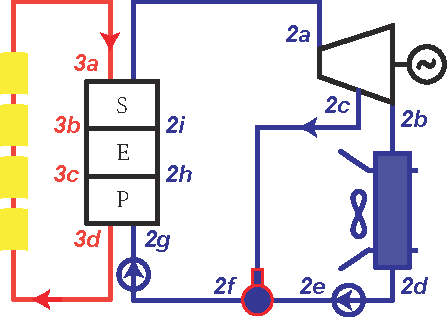
\includegraphics[width = 0.4\columnwidth]{fig/PTC}
	\caption{典型的太阳能槽式发电厂结构示意图}
	\label{fig:PTC}
\end{figure}

传统太阳能槽式电厂中的蒸汽发生系统的结构示意图见\autoref{fig:PTC}。在蒸汽发生系统中,导热油和水的流量都不发生改变。
水工质在吸热的过程中发生相变,在预热器中从过冷液体被加热成饱和液态水,在蒸发器中从饱和液态水被加热成饱和蒸汽,在过热器中从饱和蒸汽被加热成过热蒸汽。水工质的比热容在三个换热器中发生了巨大的变化。然而,由于导热油始终没有发生相变,其比热容相对变化很小。蒸汽发生系统中的传热过程曲线图如\autoref{fig:DeltaTmin}所示。

\begin{figure}[htbp]
\centering
	\includegraphics[width = 0.5\columnwidth]{fig/DeltaTmin}
	\caption{逆流布置的蒸汽发生器中的换热过程曲线}
	\label{fig:DeltaTmin}
\end{figure}

状态点$3a$的温度代表了太阳能场的出口油温,而状态点$3d$的温度代表了太阳能场的进口油温。二者之间的差异可以通过调节太阳能场中的导热油的流量来调节。

由于换热器必须保持正温差(加热流体的温度高于被加热流体的温度)工作,在蒸汽发生系统中,必须保证油温高于水温。另一方面,油温不能比水温高太多。更高的导热油温度意味着太阳能场中运行的导热油也具有更高的温度,集热器的集热效率将会下降,从而引起系统效率的下降。此外,较高的油温会给太阳能光热系统的运行带来不利的影响。因此,在蒸汽发生系统中,导热油的温度必须比水的温度高但不能高太多。设置适当的导热油和水之间的传热温差就显得格外重要。

为了确定导热油的温度,一般设计了蒸汽发生系统中导热油与水之间的最小传热温差,这个温差称为夹点温度($\Delta T_{min}$)。夹点温度一般设定为蒸发器的导热油出口温度与水的进口温度之差,即$T_{3c} - T_{2h} = \Delta T_{min}$。这是因为传统太阳能槽式电站的蒸汽发生系统中,导热油和水的温差在这里最低。太阳能槽式电站的夹点温度一般设置为10$\sim$20$\,\mathrm{K}$。
需要指出的是,需要注意温差$T_{3d} - T_{2g}$和$T_{3a} - T_{2a}$应该保持大于$\Delta T_{min}$。

然而,即使设定了蒸汽发生系统中的最小换热温差$\Delta T_{min}$,由于水存在相变,整个换热过程的平均换热温差依然很大。在\autoref{fig:DeltaTmin}中,水的$T$-$Q$曲线为折线,而导热油的$T$-$Q$曲线几乎为直线(因为导热油的比热容变化不大)。在各个换热器的进出口存在很大的温差。

虽然可以通过改变导热油的流量来改变导热油的温度,但在考虑选取导热油的流量时,需要作出折衷选择。如\autoref{fig:DeltaT}所示,改变导热油的质量流量$\dot{m}_3$会影响过程线$3a$-$3b$-$3c$-$3d$的斜率。更低的质量流量将使过程线更加陡峭,这样虽然减小了$T_{3d} - T_{2g}$,降低了预热器中的平均换热温差,但同时也升高了$T_{3a} - T_{2a}$,增加了过热器中的平均换热温差;更高的质量流量将使过程线更加平缓,这样虽然减小了$T_{3a} - T_{2a}$,降低了过热器中的平均换热温差,但同时也升高了$T_{3d} - T_{2g}$,增加了预热器中的平均换热温差。传统蒸汽发生系统的换热过程总是伴随着很高的换热温差,并因此产生大量的㶲损。基于此,本文提出了一种新型的蒸汽发生系统来减少换热温差。
\begin{figure}[htbp]
\centering
	\includegraphics[width = 0.5\columnwidth]{fig/DeltaT}
	\caption{选择导热油质量流量的折衷方案}
	\label{fig:DeltaT}
\end{figure}

\section{分段加热系统}
\label{sec:melrs}

传统蒸汽发生器的换热过程具有很大温差的原因在于,在换热过程中,水在不同换热器中的比热容差别很大,而导热油的比热容差别很小。这样在\autoref{fig:DeltaTmin}中,水工质的斜率变化很大,而导热油的斜率变化很小。导热油换热过程的斜率和水的换热过程的斜率不能保持接近,所以二者会出现较大的温差。
\begin{equation}
  \Delta Q = \dot{m} c_p\Delta T
\end{equation}

\begin{figure}[htbp]
\centering
	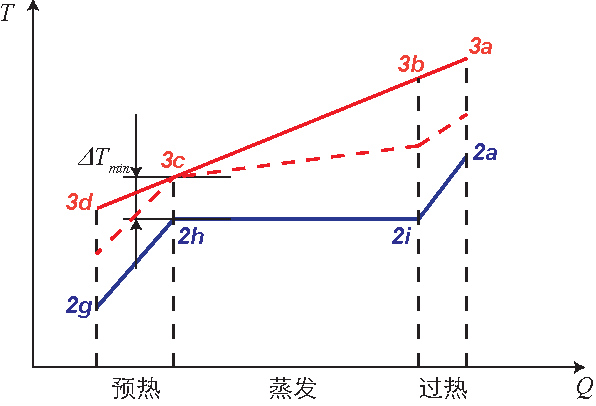
\includegraphics[width = 0.5\columnwidth]{fig/BetterCurve}
	\caption{改变各换热器中的导热油流量来减小换热温差}
	\label{fig:BetterCurve}
\end{figure}

换热曲线的斜率取决于流体的热容量$\dot{m}c_p$,所以除了比热容$c_p$的改变会导致换热曲线的斜率发生变化以外,改变流体质量流量$\dot{m}$也可以改变换热曲线的斜率。一方面,比热容属于物性参数,难以调整。另一方面,水的质量流量需要满足朗肯循环的需要,并不能随意改变。所以改变换热器中导热油的质量流量$\dot{m}_3$就成了最后一种选择。

在\autoref{fig:BetterCurve}中,导热油的换热曲线可以通过调整质量流量从实线段调整到虚线段。导热油和水的换热温差可以得到有效降低。水在三个换热器中被三股不同质量流量的导热油分段加热,所以该新的蒸汽发生系统称为分段加热系统,其太阳能槽式集热系统的结构示意图如\autoref{fig:SEP}所示。太阳能场被分成三个独立的片区。三个片区分别单独为蒸汽发生过程中的预热、蒸发和过热提供热量,且三个分区的导热油的质量流量不同。需要指出的是,\autoref{fig:SEP}中各太阳能场分区的集热器布置只是为了表示质量流量的不同。这些片区的集热器可以选取合适的数量采用串联、并联以及混联的形式进行连接。

\begin{figure}[htbp]
\centering
	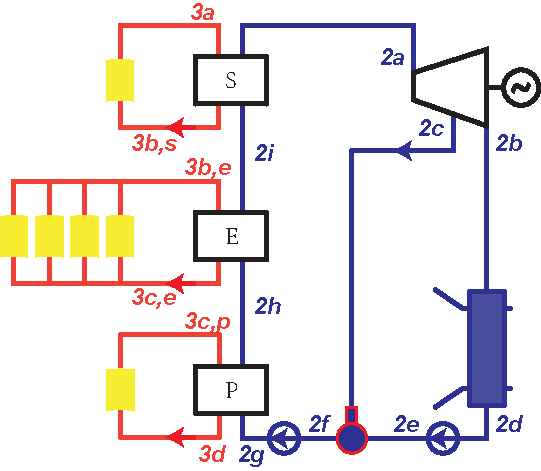
\includegraphics[width = 0.5\columnwidth]{fig/SEP}
	\caption{分段加热系统的结构示意图}
	\label{fig:SEP}
\end{figure}

值得额外说明的是,太阳能场各片区的独立性和其对应集热温度的不同给太阳能场提供了优化空间。各片区可以布置不同类型的集热器,以便于收集不同温度的热量。预热器对应的片区可以采用平板式集热器或菲涅尔反射镜来降低低温区的集热成本。蒸发器对应的片区可以选用大量槽式集热器并联连接以提高导热油的流量。由于该片区对温升的要求很低,所以可以将所有集热器并联使用,以最大限度地提高蒸发区的导热油流量。过热器对应的片区可以选用熔融盐作为太阳能槽式集热器的传热介质,这也有诸多益处。首先,熔融盐的稳定性要比导热油高很多,熔融盐的工作压力(约$2\,\mathrm{bar}$)要比导热油的工作压力(约$10\sim20\,\mathrm{bar}$)低很多,这更有利于系统的稳定运行。其次,熔融盐只运行于高温片区,降低了低温凝固的风险。最后,熔融盐作为传热介质可以克服导热油极限温度较低(约400$\,^\circ\mathrm{C}$)的缺陷,可以通过提高主汽温度提升朗肯循环的效率。针对采用分段加热系统的太阳能场的这些优化工作有待未来进一步深入研究,本文仅仅分析各片区均采用导热油为传热流体的槽式集热器的情况。

为了优化分段加热系统,考虑到夹点温度的限制,为导热油在各换热器的进出口的温度设置了以下限制条件:
\begin{eqnarray*}
	&T_{3d} = T_{2g} + \Delta T_{min}\\
   &T_{3c,p} = T_{3c,e} = T_{3c}\\
   &T_{3c} = T_{2h} + \Delta T_{min}\\
	&T_{3b,e} = T_{3b,s} = T_{3b}\\
	&T_{3a} = T_{2a} + \Delta T_{min}
\end{eqnarray*}

可以增大蒸发器中导热油的质量流量$\dot{m}_{3,e}$来减小$T_{3b}$,进而减小蒸发器中的换热温差。需要指出的是,大的流量将会导致油泵功率的增加。此外,导热油的流速还受到管道极限流速的限制(虽然采用集热器并联方案可以有效降低导热油的流速)。

导热油的每一个状态点都由温度和压力确定。为预热过程供热的太阳能场片区的最佳平均油温为
\begin{equation}
  T_{3,p} = (T_{2g} + T_{2h})/2 + \Delta T_{min}
\end{equation}

为预热过程供热的太阳能场片区的最佳导热油流量为
\begin{equation}
  \dot{m}_{3,p} = \dot{m}_{2}(h_{2h} - h_{2g})/(h_{3c} - h_{3d})
\end{equation}

为蒸发过程供热的太阳能场片区的最佳平均油温为
\begin{equation}
  T_{3,e} = (T_{3b} + T_{3c})/2
\end{equation}

为蒸发过程供热的太阳能场片区的最佳导热油流量为
\begin{equation}
  \dot{m}_{3,e} = \dot{m}_{2}(h_{2i} - h_{2h})/(h_{3b} - h_{3c})
  \label{eq:m_3e}
\end{equation}

为过热过程供热的太阳能场片区的最佳平均油温为
\begin{equation}
  T_{3,s} = (T_{3b} + T_{2a} + \Delta T_{min})/2
\end{equation}

为过热过程供热的太阳能场片区的最佳导热油流量为
\begin{equation}
  \dot{m}_{3,s} = \dot{m}_{2}(h_{2a} - h_{2i})/(h_{3a} - h_{3b})
\end{equation}

\section{对比分析}

为了更深入地研究分段加热系统,本文利用太阳能光热发电系统的部件模型,分别建立了传统型式的蒸汽发生系统和本文提出的分段加热系统的模型。
为了更加清楚地描述分段加热对太阳能场带来的影响,在研究太阳能场的效率时使用了\autoref{sec:ptc}中的\autoref{eq:eta_tc}来计算太阳能场片区导热油进出口温度对太阳能场集热效率的影响。

\begin{table}[htbp]
	\caption{传统蒸汽发生系统和分段加热系统采用的主要设计参数}
	\centering
	\begin{tabular}{p{1.5cm}<{\centering} p{3.5cm}<{\centering} p{1.5cm}<{\centering} p{3.5cm}<{\centering}}
		\toprule
		参数		&	值	&	参数		&	值\\
		\midrule
		$I_r$	&	700$\,\mathrm{W/m^2}$	&	$T_s$		&	613.15$\,\mathrm{K}$\\
		$P_{ge}$	&	6$\times$10$^6\,\mathrm{W}$	&	$p_s$		&	2.35$\times$10$^6\,\mathrm{Pa}$\\
		$\eta_{i,tb}$	&	0.711	&	$p_c$		&	1.5$\times$10$^4\,\mathrm{Pa}$\\
		$\eta_{ge}$	&	0.975	&	$p_{de}$		&	1$\times$10$^6\,\mathrm{Pa}$\\
		$\Delta T_{min}$	&	15$\,\mathrm{K}$	&	&\\		
		\bottomrule
	\end{tabular}
	\label{tab:ptc}
\end{table}

由于两个系统(传统蒸汽发生系统和分段加热系统)的汽轮机和除氧器完全相同,水循环的各状态点的参数也一样。朗肯循环的主汽参数见\autoref{tab:ptc}。

正如在\autoref{sec:melrs}中所讨论的,$T_{3b}$是未定的参数。\autoref{fig:T3b}显示了其最小值$T_{3b,min}$和最大值$T_{3b,max}$。$T_{3b,min}$表示当蒸发区导热油的流量为无穷大时,蒸发器的进口油温,$T_{3b,min} = T_{3c}$。$T_{3b,max}$和传统蒸汽发生系统在蒸发区和过热区的效果相同,即导热油在这两个区的流量相同,$\dot{m}_{3,e} = \dot{m}_{3,s}$。本文添加了另一个中间值$T_{3b}$作为参考值,$T_{3b} = (T_{3b,min} + T_{3b,max}) / 2$。
\begin{equation}
  \dfrac{T_{3b,max}-T_{3c}}{T_{3a} - T_{3c}} = \dfrac{T'_{3b} - T_{3c}}{T'_{3a} - T_{3c}}
\end{equation}
其中,$T'_{3a}$和$T'_{3b}$分别是传统蒸汽发生系统中过热器和蒸发器的进口油温。

单位时间内一个换热过程产生的㶲损由下式计算
\begin{equation}
  \dot{I} = T_{amb} (\sum \dot{m}_os_o - \sum \dot{m}_is_i)
  \label{eq:dot_I}
\end{equation}

\begin{figure}[htbp]
\centering
	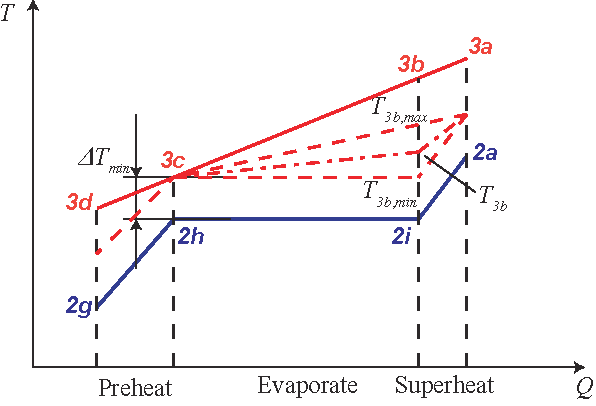
\includegraphics[width = 0.7\columnwidth]{fig/T3b}
	\caption{$T_{3b}$的取值示意图}
	\label{fig:T3b}
\end{figure}

\begin{table}[t!]
	\caption{传统蒸汽发生系统和分段加热系统的模拟结果}
	\centering
	\begin{tabular}{ccccc}
		\toprule
		& \multirow{2}{*}{传统蒸汽发生系统} & \multicolumn{3}{c}{分段加热系统}\\\cline{3-5}
 &  & $T_{3b,max}$ & $T_{3b}$ & $T_{3b,min}$\\
		\midrule
		$T_{2a}$ & \multicolumn{4}{c}{613.15$\,\mathrm{K}$}\\
		$T_{2i}$ & \multicolumn{4}{c}{493.83$\,\mathrm{K}$}\\
		$T_{2h}$ & \multicolumn{4}{c}{493.83$\,\mathrm{K}$}\\
		$T_{2g}$ & \multicolumn{4}{c}{453.28$\,\mathrm{K}$}\\
		$T_{3c}$ & \multicolumn{4}{c}{508.83$\,\mathrm{K}$}\\
%		$T_{3d}$	&	495.43$\,\mathrm{K}$	&	\multicolumn{3}{c}{468.28$\,\mathrm{K}$}\\
		$T_{3a}$	&	653.15$\,\mathrm{K}$
	&	628.15$\,\mathrm{K}$	&	628.15$\,\mathrm{K}$	&	628.15$\,\mathrm{K}$\\
		$T_{3b}$	&	634.11$\,\mathrm{K}$	&	612.41$\,\mathrm{K}$	&	560.62$\,\mathrm{K}$	&	508.83$\,\mathrm{K}$\\
		$T_{3d}$	&	495.43$\,\mathrm{K}$
	&	468.28$\,\mathrm{K}$	&	468.28$\,\mathrm{K}$	&	468.28$\,\mathrm{K}$\\
%		$T_{3a}$	&	653.15$\,\mathrm{K}$	&	\multicolumn{3}{c}{628.15$\,\mathrm{K}$}\\
		$\dot{m}_{3p}$	&	47.8$\,\mathrm{kg/s}$	&	16.1$\,\mathrm{kg/s}$	&	16.1$\,\mathrm{kg/s}$	&	16.1$\,\mathrm{kg/s}$\\
		$\dot{m}_{3e}$	&	47.8$\,\mathrm{kg/s}$	&	58.6$\,\mathrm{kg/s}$	&	120.8$\,\mathrm{kg/s}$	&	$\infty$\\
		$\dot{m}_{3s}$	&	47.8$\,\mathrm{kg/s}$	&	59.4$\,\mathrm{kg/s}$	&	14.3$\,\mathrm{kg/s}$	&	8.3$\,\mathrm{kg/s}$\\
		$\dot{I}_p$    &    4.80$\times$10$^4\,\mathrm{W}$    	&  2.58$\times$10$^4\,\mathrm{W}$  &	2.58$\times$10$^4\,\mathrm{W}$	&	2.58$\times$10$^4\,\mathrm{W}$\\
		$\dot{I}_e$    &    1.10$\times$10$^6\,\mathrm{W}$    	&  9.68$\times$10$^5\,\mathrm{W}$  &	6.24$\times$10$^5\,\mathrm{W}$	&	2.41$\times$10$^5\,\mathrm{W}$	\\
		$\dot{I}_s$    &    1.81$\times$10$^5\,\mathrm{W}$    	&  1.42$\times$10$^5\,\mathrm{W}$  &	9.19$\times$10$^4\,\mathrm{W}$	&	4.24$\times$10$^4\,\mathrm{W}$\\
		$\dot{I}_{total}$    &    1.33$\times$10$^6\,\mathrm{W}$    &  1.14$\times$10$^6\,\mathrm{W}$  &	7.44$\times$10$^5\,\mathrm{W}$	&	3.10$\times$10$^5\,\mathrm{W}$\\
		$\eta_p$    &    0.699    &	0.703	&    0.703	&	0.703\\
		$\eta_e$    &    0.673    &	0.678	& 0.689	&	0.697\\
		$\eta_s$    &    0.633    &  0.648	&  0.662	&	0.675\\
		$\eta_{overall}$    &    0.670   &	0.676	&    0.686	&	0.695\\
		\bottomrule
	\end{tabular}
	\label{tab:comparison}
\end{table}
%该表格的解释

传统蒸汽发生系统及三种分段加热系统的模型的模拟结果见\autoref{tab:comparison}。可以发现,分段加热系统可以有效降低蒸汽发生过程中产生的㶲损。三种方案的㶲损可以减少14.3\%到76.7\%。太阳能场的集热效率可以提升0.9\%到3.6\%。

需要指出的是,对于$T_{3b} = T_{3b,min}$的方案,当蒸发区的导热油的质量流量趋于无穷大时,\autoref{eq:dot_I}不再适用。这时采用等温换热过程的计算公式来计算单位时间的㶲损
\begin{equation}
  \dot{I} = T_{amb} (\frac{\dot{Q}}{T_{2h}} - \frac{\dot{Q}}{T_{3c}}) = \frac{\dot{Q}T_{amb}(T_{3c} - T_{2h})}{T_{2h}T_{3c}}
  \label{eq:isothermal}
\end{equation}
其中,$\dot{Q}$是蒸发过程中单位时间内传递的热量。

由于水回路相同,四种系统的$T_{2a}$、$T_{2i}$、$T_{2h}$、$T_{2g}$和$T_{3c}$都相同。油回路的流量各不相同,这导致了不同的油水换热温差,并因此带来不同的㶲损。从表中可以发现,改变导热油的流量可以有效降低整个换热过程中的㶲损。分段加热系统的预热器中的㶲损值($2.58\times 10^4\,\mathrm{W}$)要小于传统蒸汽发生系统的㶲损值($4.80\times10^4\,\mathrm{W}$)。不同分段加热系统的蒸发器中的㶲损值差别很大,当导热油的流量从$58.6\,\mathrm{kg/s}$增加到无穷大时,㶲损从$9.68\times10^5\,\mathrm{W}$降到$2.41\times10^5\,\mathrm{W}$。
蒸发器中的㶲损占整个蒸汽发生系统中的㶲损的最大比例,不同系统中的占比在78.0\%到85.2\%之间。不同分段加热器的过热器的㶲损值($1.42\times 10^5\,\mathrm{W}$、 $9.19\times 10^4\,\mathrm{W}$及$4.24\times 10^4\,\mathrm{W}$)要远小于传统蒸汽发生系统的㶲损值($1.81\times10^5\,\mathrm{W}$)。

上述结果还表明,采用分段加热系统可以有效降低蒸汽发生过程中导热油的平均温度,提升各片区的集热效率,太阳能场的总体集热效率可以得到有效提升。三种分段加热系统方案可使太阳能场的集热效率提升0.9\%到3.6\%。

\section{本章小结}

针对传统蒸汽发生系统中存在较大㶲损的问题,本文提出了分段加热系统。
该系统将传统的太阳能场分成了独立的三个片区来分别为预热过程、蒸发过程和过热过程提供热量。不同片区具有不同的导热油流量,来控制各换热过程的换热温差。

通过给各片区设置合适的导热油流量,可以有效降低各换热过程的换热温差。较低的换热温差意味着较低的导热油温度,这有利于提高太阳能场的集热效率。此外,太阳能场各片区的独立性和集热温度的差异也给太阳能场的优化提供了空间。给不同的片区配置不同类型的集热器是提高系统效率的一条可行方案。

为了精确描述本文提出的分段加热系统相比于传统蒸汽发生系统的优越性,本文建立了各类系统的模型,并提出了各片区导热油流量的控制策略。利用所建立的模型,对各系统进行了效率分析和㶲分析。结果表明,本文提出的分段加热方法能够有效降低蒸汽发生过程中产生的㶲损,系统的效率也会得到相应的提高。与传统的蒸汽发生系统相比,三种不同方案可使蒸汽发生过程的㶲损失减少14.3\%到76.7\%,太阳能场的集热效率也会提高0.9\%到3.6\%。